% -*-cap2.tex-*-
% Este fichero es parte de la plantilla LaTeX para
% la realización de Proyectos Final de Carrera, protegido
% bajo los términos de la licencia GFDL.
% Para más información, la licencia completa viene incluida en el
% fichero fdl-1.3.tex

% Copyright (C) 2009 Pablo Recio Quijano 

% MANUAL DE USUARIO

% FIXME
% subir al apartado de ficheros de RedIRIS los manuales

\section{Ejecución}

En este capítulo veremos el funcionamiento de la aplicación desde el punto de vista de un usuario final que ejecutará el
videojuego con la intención de disfrutar de las opciones que ofrece. \\

Si el programa está instalado, se ejecuta con:

\begin{lstlisting} [language=Bash, numbers=left]
user@machine:~$ python dominous.py
\end{lstlisting}

o con un simple doble click si nos encontramos en un entorno windows. \\


\section{Menú principal}

\begin{figure}[h]
  \label{fig:screenshots_menu}
  \begin{center}
    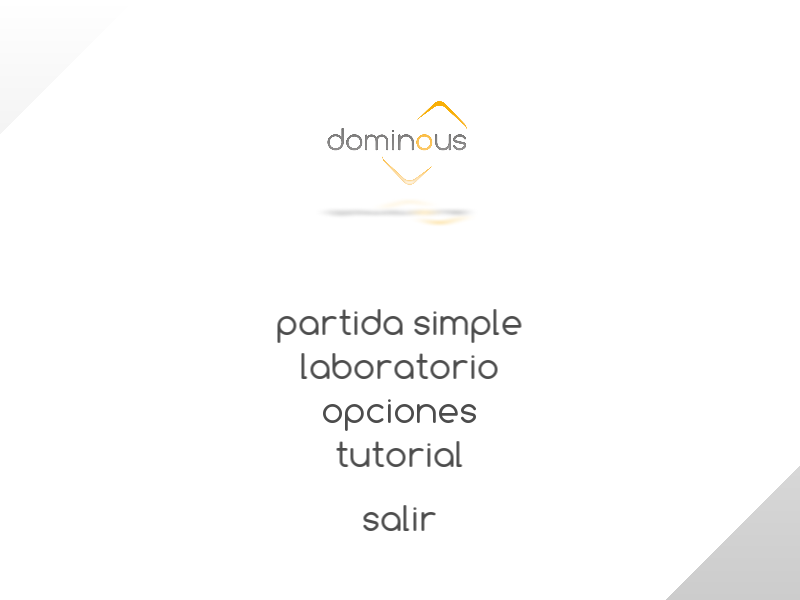
\includegraphics[scale=0.8]{screenshots_menu.png}
  \end{center}
  \caption{Menú principal de Dominous}
\end{figure}

El menú principal~\ref{fig:screenshots_menu} ofrece las siguientes opciones:

\begin{description}
    \item[Partida simple] Será la poción más utilizada, ya que permite al usuario disfrutar de una partida de dominó.
    \item[Laboratorio] El modo laboratorio enfrenta a dos equipos controlados por el ordenador a cien partidas, para
            intentar dilucidar qué equipo es mejor.
    \item[Opciones] Las opciones del juego nos permite configurar la partida a nuestras necesidades, como veremos en el
            siguiente apartado.
    \item[Tutorial] Nos muestra un conjunto de diapositivas o transparencias con información rápida sobre cómo jugar,
            qué nos ofrece Dominous y unas breves nociones de juego del dominó.
    \item[Salir] Cierra y sale del juego.
\end{description}

Para movernos entre las distintas opciones simplemente debemos utilizar el ratón e ir clicando en las diferentes secciones,
pulsando el botón volver para retornar al menú principal en cualquier momento. Continuemos el manual mostrando la sección
tutorial y viendo las opciones que nos ofrece.


\section{Opciones}

Las opciones de juego~\ref{fig:screenshots_options}, tal y como hemos comentado previamente, nos permite adaptar diferentes opciones de Dominous según
nuestras necesidades. Las opciones que se muestran son las siguientes:

\begin{figure}[h]
  \label{fig:screenshots_options}
  \begin{center}
    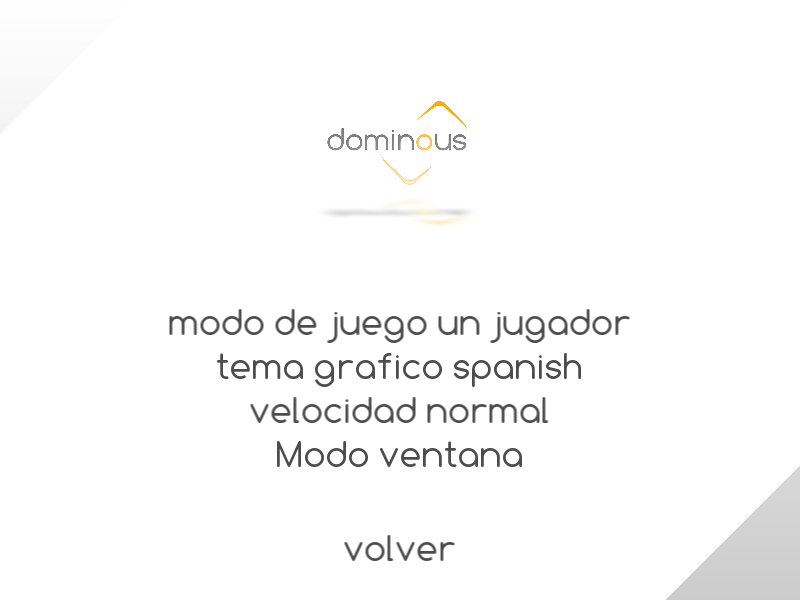
\includegraphics[scale=0.8]{screenshots_options.png}
  \end{center}
  \caption{Pantalla de opciones de juego}
\end{figure}

\begin{description}
    \item[Modo de juego] Podemos seleccionar si, en el modo de juego \textbf{partida simple}, queremos participar nosotros
        como jugador activo o simplemente queremos observar cómo el ordenador desarrolla la partida completa, controlando
        él mismo a todos los jugadores. 
    \item[Tema gráfico] Esta opción nos permite seleccionar el aspecto gráfico de la partida~\ref{fig:screenshots_themes}.
        El aspecto gráfico permite cambiar la visualización de fichas, mesa de juego y otros elementos, al estilo de los
        temas gráficos que poseen otros programas o los sistemas operativos, por ejemplo.
    \item[Velocidad de juego] Dominous posee tres tipos de velocidades de juego:
        \begin{itemize}
            \item Velocidad normal --- el juego se desarrolla a una velocidad pausada, con movimientos de fichas que permiten
                seguir el transcurso de la partida con comodidad, y se muestra información sobre el tiempo que emplea cada
                jugador mientras piensa la jugada a ejecutar.
            \item Velocidad rápida --- las fichas se mueven a la misma velocidad que en el modo normal, pero los jugadores
                colocan la ficha inmediatamente en cuanto les toca su turno.
            \item Velocidad extra rápida --- el movimiento de las fichas es acelerado y los jugadores no emplean tiempo
                pensando la jugada.
        \end{itemize}
    \item[Modo ventana] Por último, esta opción nos permite cambiar el modo de juego de ventana a modo pantalla completa.
            Solamente recordar, como se indica en el menú, que es necesario reiniciar el juego para que este cambio
            concreto se lleve a cabo.
\end{description}

\begin{figure}[h]
  \label{fig:screenshots_themes}
  \begin{center}
    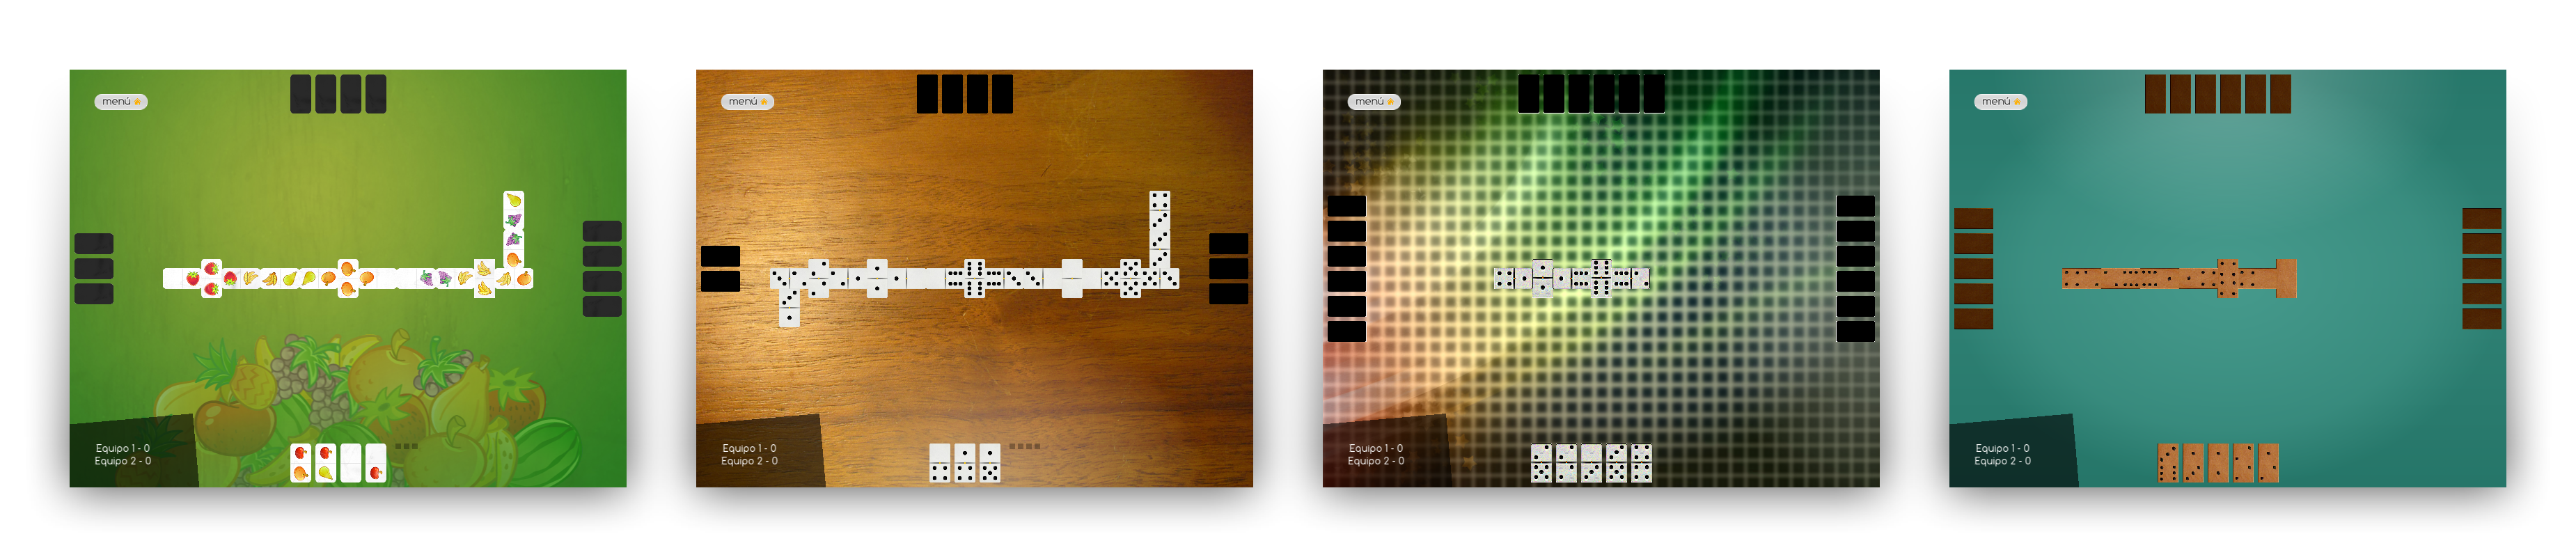
\includegraphics[scale=0.15]{screenshots_themes.png}
  \end{center}
  \caption{Diferentes temas gráficos que vienen de serie con Dominous}
\end{figure}


\section{Tutorial}

El tutorial de juego~\ref{fig:screenshots_tutorial} sirve de ayuda a los nuevos jugadores de Dominous, presentando de forma
resumida todas las opciones que posee Dominous y evitando que, en un primer uso, sea necesario leer todo el manual de usuario.

\begin{figure}[h]
  \label{fig:screenshots_tutorial}
  \begin{center}
    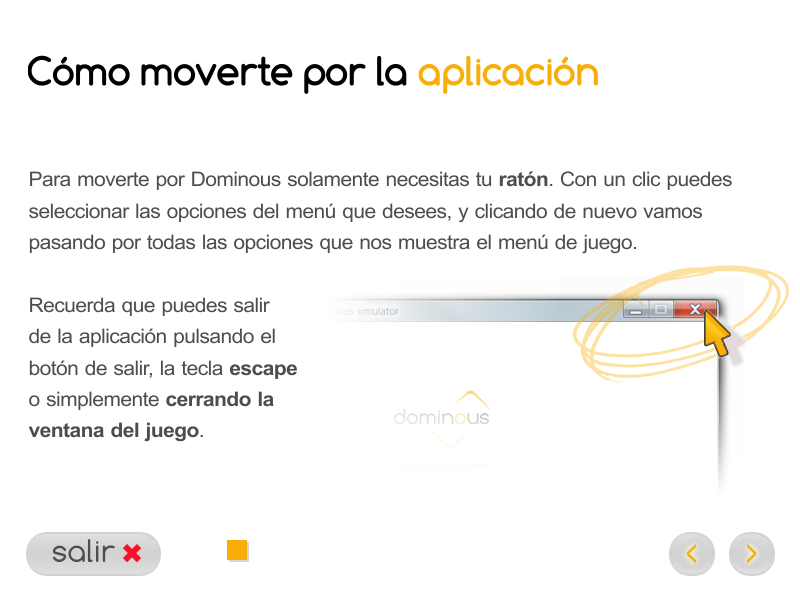
\includegraphics[scale=0.8]{screenshots_tutorial.png}
  \end{center}
  \caption{Modo tutorial, con instrucciones básicas de juego}
\end{figure}

\begin{itemize}
    \item Las primeras capturas informan sobre la interfaz de Dominous: cómo moverte por las opciones, salir del juego, jugar
        una partida, colocar fichas, entrar y salir de una partida de dominó, y diferentes elementos que se muestran a la
        hora de disfrutar de una partida.
    \item Luego se nos informa del modo Laboratorio, describiendo cada uno de los elementos que aparecen en pantalla como
        son las barras de información o la gráfica de partidas ganadas.
    \item Por último se pretende dar al usuario novel de unas nociones básicas de dominó: cómo jugar, cuántas fichas existen,
        breve explicación sobre el modo de juego por parejas y cierres.
\end{itemize}


\section{Jugando una partida a Dominous}

La opción \textbf{partida simple} nos dirige directamente a disfrutar de una partida de dominó por parejas. La primera
pantalla que se nos muestra es la de selección de jugadores~\ref{fig:screenshots_select_players_game}, en la que debemos
decidir nuestra pareja de equipo y los dos jugadores contra los que nos vamos a enfrentar. \\

Nuestra posición en la mesa viene determinada por una figura gris con el texto \textbf{jugador 1} y un icono indicando
que este jugador estará controlado por el ratón; siguiendo con las normas clásicas de dominó, nuestra pareja estará situada
justo enfrente de nosotros (jugador situado en la zona superior de la pantalla) y nuestros adversarios estarán colocados
a izquierda y derecha de nuestra posición. \\

\begin{figure}[h]
  \label{fig:screenshots_select_players_game}
  \begin{center}
    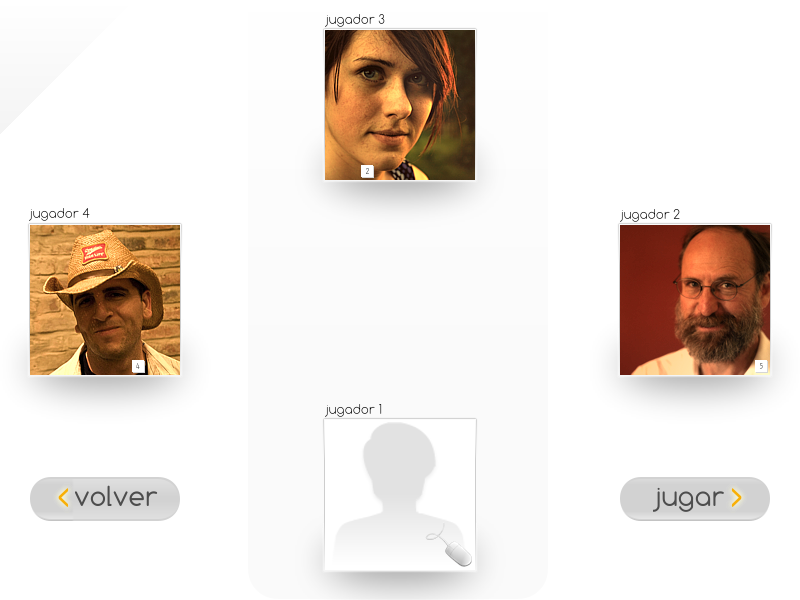
\includegraphics[scale=0.8]{screenshots_select_players_game.png}
  \end{center}
  \caption{Pantalla de selección de pareja de equipo y contrincantes}
\end{figure}

Para elegir pareja o adversario simplemente tenemos que pulsar encima del avatar correspondiente, y el jugador seleccionado
irá rotando de entre todos los jugadores disponibles en la biblioteca. \\

Una vez elegidos los jugadores, pulsamos el botón jugar, y dará comienzo la partida mostrándose algo similar --- dependiendo
del tema gráfico seleccionado --- a la siguiente imagen~\ref{fig:screenshots_game}. \\

\begin{figure}[h]
  \label{fig:screenshots_game}
  \begin{center}
    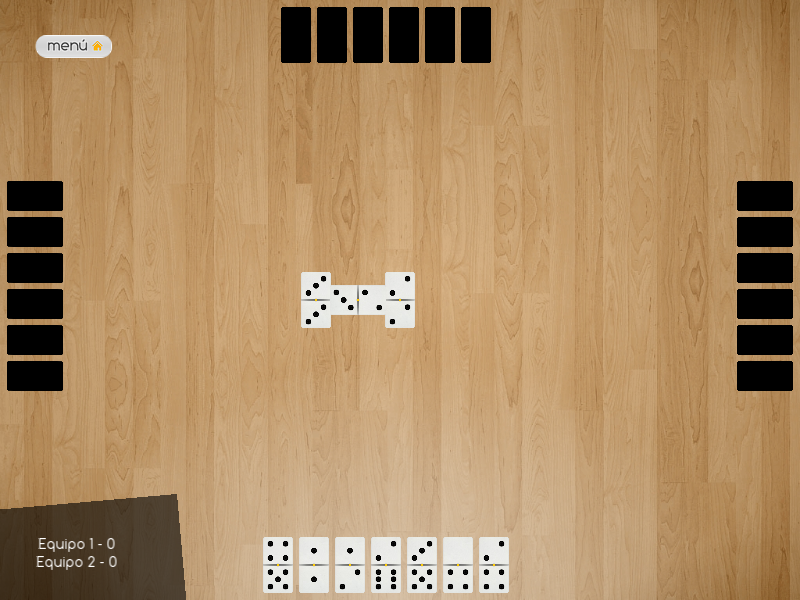
\includegraphics[scale=0.8]{screenshots_game.png}
  \end{center}
  \caption{Pantalla principal de juego}
\end{figure}

Nuestra posición en la mesa está situada en la parte inferior, con las fichas boca arriba para poder verlas cómodamente. El
turno de cada jugador se indica con una marca que rodea las fichas; en este caso vemos como un aura o sombra blanca rodea
las fichas del jugador 1, por lo tanto es nuestro turno para colocar ficha. \\

Las fichas se colocan simplemente arrastrando y soltando la ficha cerca de la zona que deseemos, es decir, debemos:
\begin{enumerate}
    \item Colocamos el ratón sobre la ficha que queremos colocar, y pulsamos (sin soltarlo) el botón izquierdo del ratón.
    \item Movemos el ratón y la ficha cerca de la zona en la que queremos colocar la ficha.
    \item Soltamos el botón izquierdo del ratón.
\end{enumerate}

Si hemos llevado con éxito la tarea, la ficha se colocará suavemente en su sitio. Por el contrario, si hemos soltado la ficha
en un lugar no permitido o la ficha no era una candidata viable a ser colocada, volverá suavemente a su sitio y deberemos
volver a intentarlo. \\

La partida se desarrolla hasta que se dan alguna de las circunstancias por las que puede terminar --- se produce un cierre o 
un jugador se queda sin fichas --- y en ese momento se muestra la pantalla de suma de puntos~\ref{fig:screenshots_game_finish},
en la que se muestran boca arriba las fichas de los dos equipos y se suman los puntos para saber quién es el ganador (en caso
de cierre) o cuántos puntos se suma el equipo que ha ganado la mano.

\begin{figure}[h]
  \label{fig:screenshots_game_finish}
  \begin{center}
    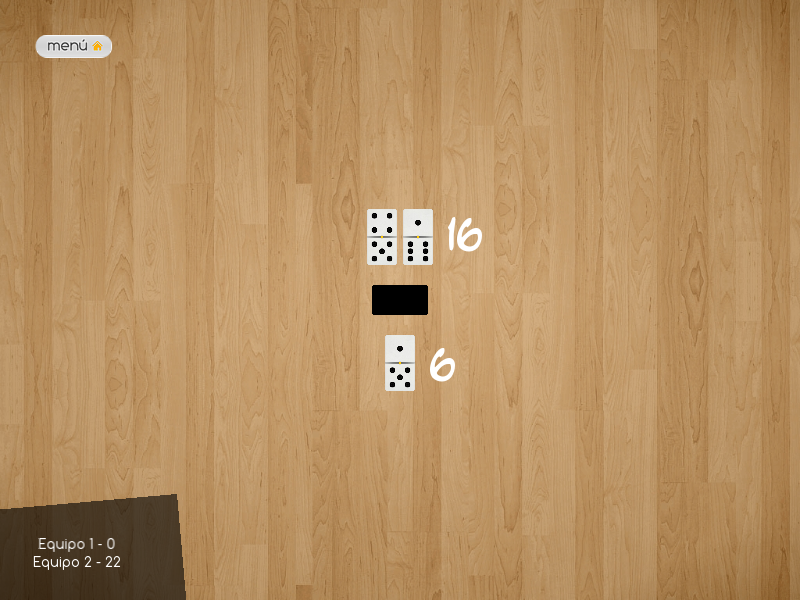
\includegraphics[scale=0.8]{screenshots_game_finish.png}
  \end{center}
  \caption{Se suman las fichas de los integrantes de cada equipo, comparando y sumándolo al equipo ganador}
\end{figure}

Por último aparece la pantalla de puntos totales~\ref{fig:screenshots_game_finish2}, con un listado de los resultados de
todas las manos del juego hasta el momento, y el equipo que lleva ventaja en el marcador se muestra destacado en amarillo.

\begin{figure}[h]
  \label{fig:screenshots_game_finish2}
  \begin{center}
    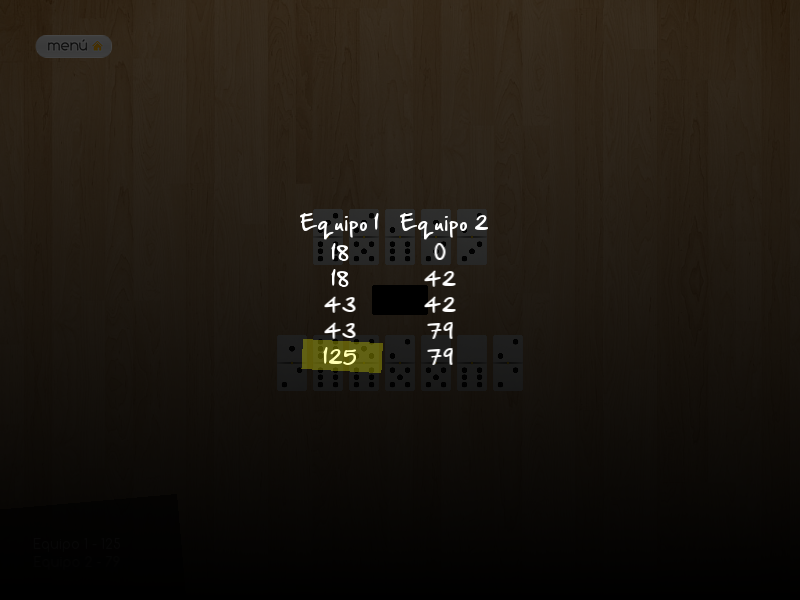
\includegraphics[scale=0.8]{screenshots_game_finish2.png}
  \end{center}
  \caption{Listado con la puntuación de todas las manos del juego}
\end{figure}

Pulsando cualquier botón continuamos con el juego, dando comienzo una nueva mano. \\

La dinámica del juego continúa hasta que uno de los dos equipos alcanza o supera los 200 puntos, momento en el cual se
muestra la última pantalla de resumen de puntos y a continuación, con letras titulares, el equipo ganador del
encuentro~\ref{fig:screenshots_game_finish3}. Para terminar pulsamos cualquier tecla y volvemos al menú de inicio.

\begin{figure}[h]
  \label{fig:screenshots_game_finish3}
  \begin{center}
    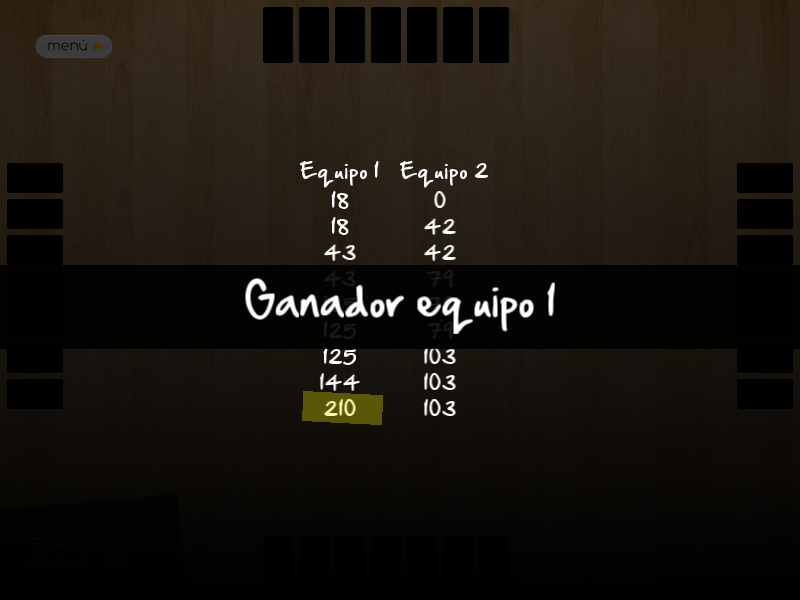
\includegraphics[scale=0.8]{screenshots_game_finish3.png}
  \end{center}
  \caption{El equipo 1 ha ganado el encuentro}
\end{figure}


\section{Modo laboratorio}

Lorem ipsum
